\documentclass[12pt]{article}

% ============================================================
%  Template SBC (Sociedade Brasileira de Computacao)
%  Use no Overleaf: "SBC Conference Template" (fornece sbc-template.sty)
%  ou coloque o arquivo sbc-template.sty na mesma pasta deste main.tex.
%  Enunciado: ate 8 paginas, SEM abstract/resumo.
% ============================================================

\usepackage{sbc-template}
\usepackage{graphicx,url}
\usepackage[utf8]{inputenc}
\usepackage[brazil]{babel}
\usepackage{booktabs}
\usepackage{multirow}
\usepackage{float}

\sloppy

\title{Classificação de Personagens da Série \textit{The Simpsons} com
\textit{Deep Features} e Fusão Estática de Classificadores}

\author{Autor Um\inst{1}, Autor Dois\inst{1}}

\address{Departamento de Computação (DACOM) -- Universidade Tecnológica
Federal do Paraná (UTFPR)\\
Campus Campo Mourão -- Campo Mourão -- PR -- Brasil
\email{\{autor1,autor2\}@alunos.utfpr.edu.br}
}

\begin{document}

\maketitle

% ============================================================
\section{Introdução}
% ============================================================

O reconhecimento automático de personagens em imagens é um problema clássico
de visão computacional que combina extração de características visuais e
classificação supervisionada. Neste trabalho aborda-se a classificação de cinco
personagens da família principal da série \textit{The Simpsons} --- Bart, Homer,
Lisa, Maggie e Marge --- a partir de imagens estáticas. O desafio é relevante
porque as classes apresentam forte semelhança de paleta de cores e traços
visuais (tom amarelo da pele, contornos simples), além de desbalanceamento entre
classes, o que torna o problema sensível tanto à qualidade do descritor de
características quanto à robustez do classificador.

A proposta deste trabalho é um \textit{pipeline} de classificação que (i) extrai
\textit{deep features} de um modelo pré-treinado \textit{Vision Transformer}
(ViT-large), (ii) avalia um conjunto de 20 classificadores cobrindo cinco
famílias distintas (k-NN, Árvore de Decisão, SVM, \textit{Random Forest} e MLP)
e (iii) aplica métodos de \textbf{fusão estática de classificadores}
(\textit{voting}, \textit{weighted voting}, \textit{Top-K ensemble} e
\textit{stacking}) para superar o melhor classificador individual. O sistema é
avaliado em dois protocolos complementares: validação cruzada de 10
\textit{folds} sobre o conjunto de treino e avaliação \textit{holdout} sobre o
conjunto de validação fornecido com a base. Reportam-se acurácia, \textit{F1-score}
macro e matrizes de confusão, além de uma análise do impacto da fusão e dos
pontos fortes e fracos do sistema.

% ============================================================
\section{Materiais e Métodos}
% ============================================================

\subsection{Base de Dados}

A base \textit{Simpsons} utilizada é composta por imagens no formato BMP,
divididas em cinco classes correspondentes aos personagens. Adotou-se a divisão
proposta nos próprios arquivos da base: um conjunto de \textbf{treino} com 226
imagens e um conjunto de \textbf{validação} (\textit{holdout}) com 95 imagens.
A Tabela~\ref{tab:base} apresenta a distribuição de imagens por classe no
conjunto de treino, evidenciando o desbalanceamento (Bart é a classe majoritária
e Maggie/Marge as minoritárias).

\begin{table}[H]
\centering
\caption{Distribuição de imagens por classe no conjunto de treino.}
\label{tab:base}
\begin{tabular}{lccccc}
\toprule
Classe & Bart & Homer & Lisa & Maggie & Marge \\
\midrule
\textit{Imagens (treino)} & 78 & 61 & 33 & 30 & 24 \\
\bottomrule
\end{tabular}
\end{table}

\subsection{Extração de Características (\textit{Deep Features})}

Em vez de descritores manuais (cor, textura, forma), optou-se por
\textbf{\textit{deep features}}: representações extraídas de uma rede neural
profunda pré-treinada, usadas como vetor de características de entrada para
classificadores clássicos. Empregou-se o modelo \textit{Vision Transformer}
\texttt{google/vit-large-patch16-224-in21k}, pré-treinado no ImageNet-21k.

Cada imagem é redimensionada e normalizada conforme o pré-processamento do
modelo; a partir da saída \texttt{last\_hidden\_state} do ViT calcula-se a média
ao longo dos \textit{tokens} (\textit{mean pooling}), gerando um vetor de
\textbf{1024 características} por imagem. Esse vetor é então padronizado
(\textit{z-score}, \texttt{StandardScaler}) com estatísticas estimadas
exclusivamente no conjunto de treino, evitando vazamento de informação para a
validação. A escolha do ViT-large justifica-se por capturar relações globais na
imagem via atenção, produzindo representações altamente discriminativas mesmo com
poucos exemplos de treino por classe.

\subsection{Classificadores}

Construiu-se um \textit{pool} de \textbf{20 classificadores} que cobre as cinco
famílias vistas na disciplina, variando hiperparâmetros relevantes
(Tabela~\ref{tab:clf}). Todos os modelos foram implementados com a biblioteca
\textit{scikit-learn}.

\begin{table}[H]
\centering
\caption{\textit{Pool} de 20 classificadores e seus hiperparâmetros.}
\label{tab:clf}
\begin{tabular}{lp{8.5cm}}
\toprule
Família & Variações \\
\midrule
k-NN & $k \in \{1,3,5,7\}$ \\
Árvore de Decisão & profundidade $\in \{5,10,15\}$; critério \textit{entropy} \\
SVM & RBF com $C \in \{0{,}1;\,1{,}0;\,10{,}0\}$; \textit{kernel} linear \\
\textit{Random Forest} & $\{10,50,100,200\}$ árvores \\
MLP & topologias $(50)$, $(100)$, $(50,25)$, $(100,50)$ \\
\bottomrule
\end{tabular}
\end{table}

\subsection{Fusão Estática de Classificadores}

Para explorar a complementaridade entre os modelos, aplicaram-se cinco
estratégias de combinação estática sobre o \textit{pool} de 20 classificadores:

\begin{itemize}
  \item \textbf{Hard Voting}: voto majoritário entre as predições de classe.
  \item \textbf{Soft Voting}: média das probabilidades \textit{a posteriori}.
  \item \textbf{Weighted Soft Voting}: \textit{soft voting} ponderado pela
        acurácia individual de cada classificador (modelos melhores pesam mais).
  \item \textbf{Top-K Ensemble}: \textit{soft voting} apenas com os $K$ melhores
        classificadores ($K \in \{5,8,10,12,15\}$), descartando modelos fracos.
  \item \textbf{Stacking}: meta-aprendizado em que uma Regressão Logística
        (nível 1) é treinada sobre as predições dos 20 classificadores (nível 0),
        com \textit{passthrough} das características originais.
\end{itemize}

\subsection{Protocolo de Avaliação e Métricas}

Adotaram-se dois protocolos: \textbf{(A) Teste} via validação cruzada
estratificada de 10 \textit{folds} sobre o treino e \textbf{(B) Validação} via
\textit{holdout}, treinando no conjunto de treino completo e avaliando no
conjunto de validação. As métricas reportadas são acurácia, \textit{F1-score}
macro (média não-ponderada por classe, adequada a bases desbalanceadas) e a
matriz de confusão $N\times N$ ($N=5$) em percentual de acertos/erros por classe.

% ============================================================
\section{Resultados e Discussão}
% ============================================================

\subsection{Classificadores Individuais (Protocolo A --- 10-fold CV)}

A Tabela~\ref{tab:ind} apresenta o desempenho dos 20 classificadores na validação
cruzada de 10 \textit{folds}. A Figura~\ref{fig:acc} mostra o comparativo visual
de acurácia (com os \textit{baselines} de fusão) e a Figura~\ref{fig:fam} a média
por família.

\begin{table}[H]
\centering
\caption{Acurácia e \textit{F1-score} macro dos classificadores individuais
(10-fold CV). Em destaque, os três melhores.}
\label{tab:ind}
\begin{tabular}{lcc}
\toprule
Classificador & Acurácia (\%) & F1-macro (\%) \\
\midrule
\textbf{MLP (50)}      & \textbf{88,05} & \textbf{86,85} \\
\textbf{SVM-Linear}    & \textbf{87,61} & \textbf{87,45} \\
\textbf{MLP (100,50)}  & \textbf{87,61} & \textbf{86,48} \\
MLP (100)              & 85,84 & 85,90 \\
SVM-RBF (C=10,0)       & 84,51 & 83,44 \\
MLP (50,25)            & 82,74 & 82,99 \\
SVM-RBF (C=1,0)        & 81,86 & 81,63 \\
kNN (k=3)              & 81,86 & 80,51 \\
RF (200 árvores)       & 79,65 & 76,69 \\
kNN (k=5)              & 79,20 & 75,14 \\
RF (100 árvores)       & 78,76 & 75,34 \\
kNN (k=1)              & 77,88 & 77,11 \\
kNN (k=7)              & 77,88 & 74,81 \\
RF (50 árvores)        & 74,78 & 69,19 \\
RF (10 árvores)        & 66,37 & 60,10 \\
DT (prof=10)           & 49,12 & 45,01 \\
DT (entropy)           & 49,12 & 43,48 \\
DT (prof=15)           & 49,12 & 45,01 \\
DT (prof=5)            & 46,90 & 42,20 \\
SVM-RBF (C=0,1)        & 34,51 & 10,26 \\
\bottomrule
\end{tabular}
\end{table}

Observa-se que as famílias \textbf{MLP} e \textbf{SVM} dominam o ranking, com o
melhor classificador individual (MLP com camada de 50 neurônios) atingindo
\textbf{88,05\%} de acurácia. As \textbf{Árvores de Decisão} isoladas são o ponto
fraco (\,$\approx$49\%\,), por não explorarem a alta dimensionalidade das
\textit{deep features} de forma robusta, e o SVM-RBF com $C=0{,}1$ colapsa
(34,51\%) por regularização excessiva. Esse contraste evidencia a importância da
escolha de hiperparâmetros e motiva a fusão, que pode tanto agregar a força dos
melhores modelos quanto ser penalizada pela inclusão dos fracos.

\begin{figure}[H]
\centering
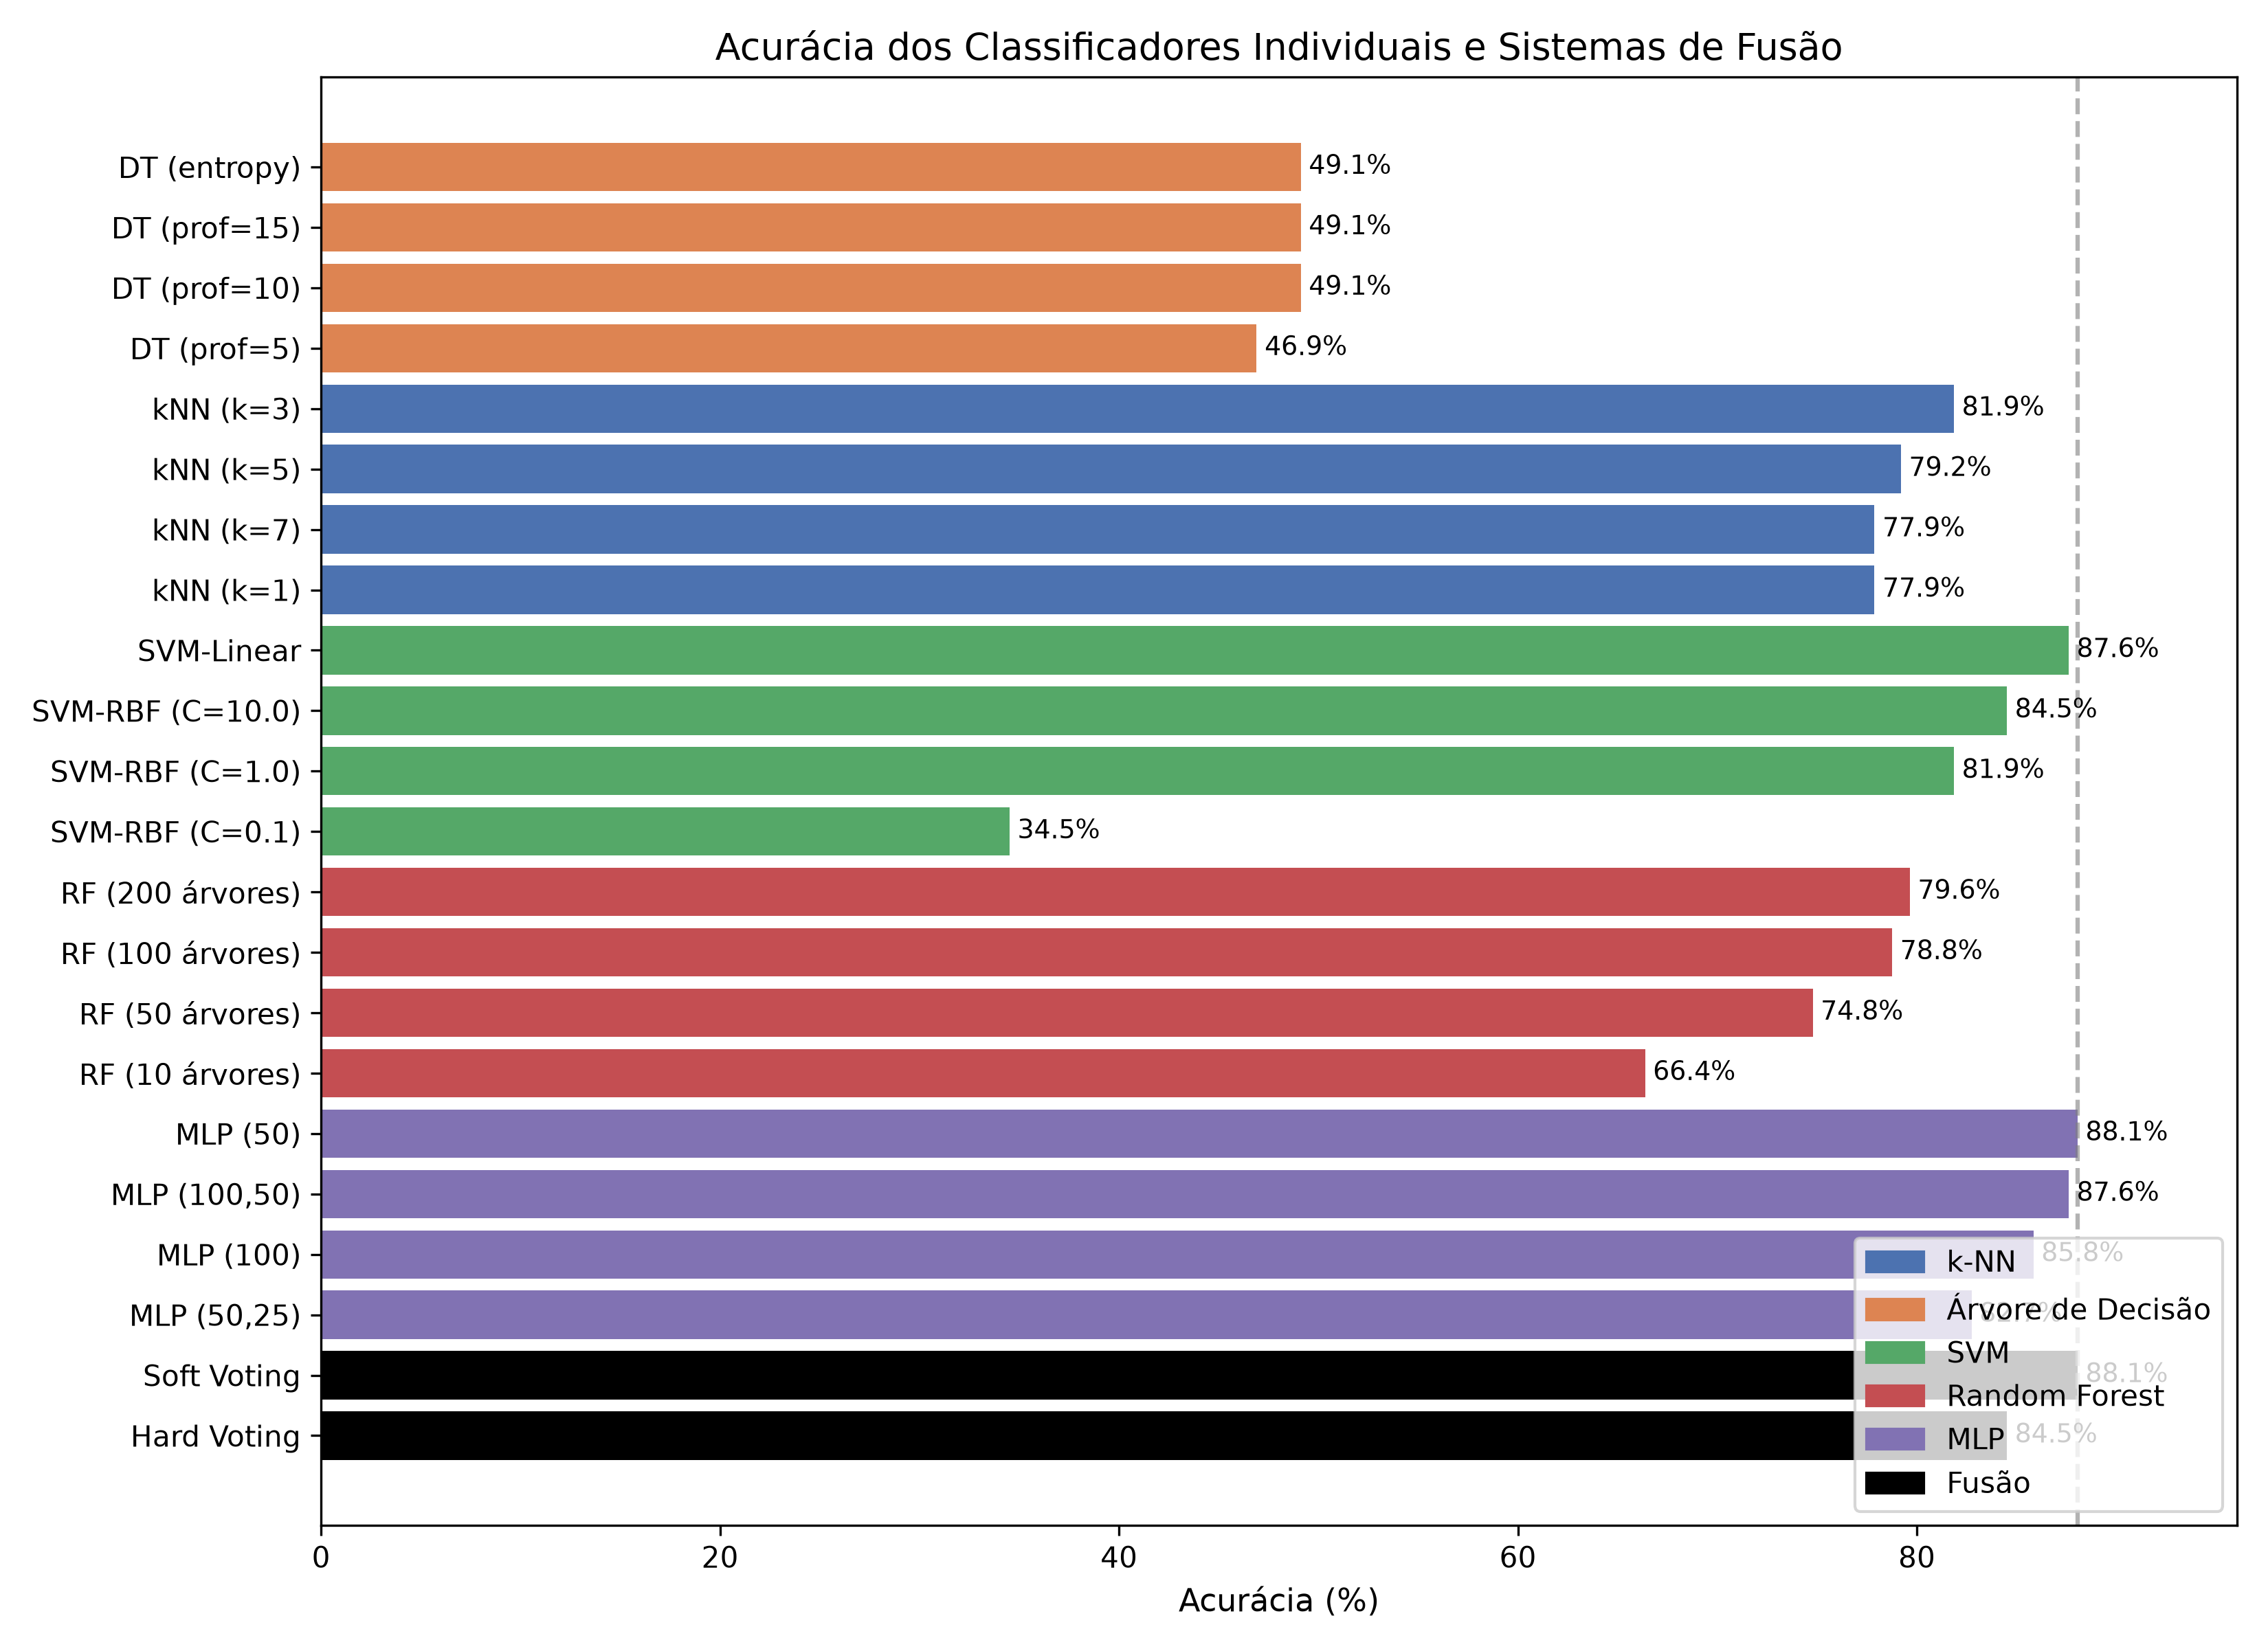
\includegraphics[width=0.78\textwidth]{figs/fig1_comparativo_acuracia.png}
\caption{Acurácia dos 20 classificadores individuais e dos \textit{baselines} de
fusão (10-fold CV), coloridos por família.}
\label{fig:acc}
\end{figure}

\begin{figure}[H]
\centering
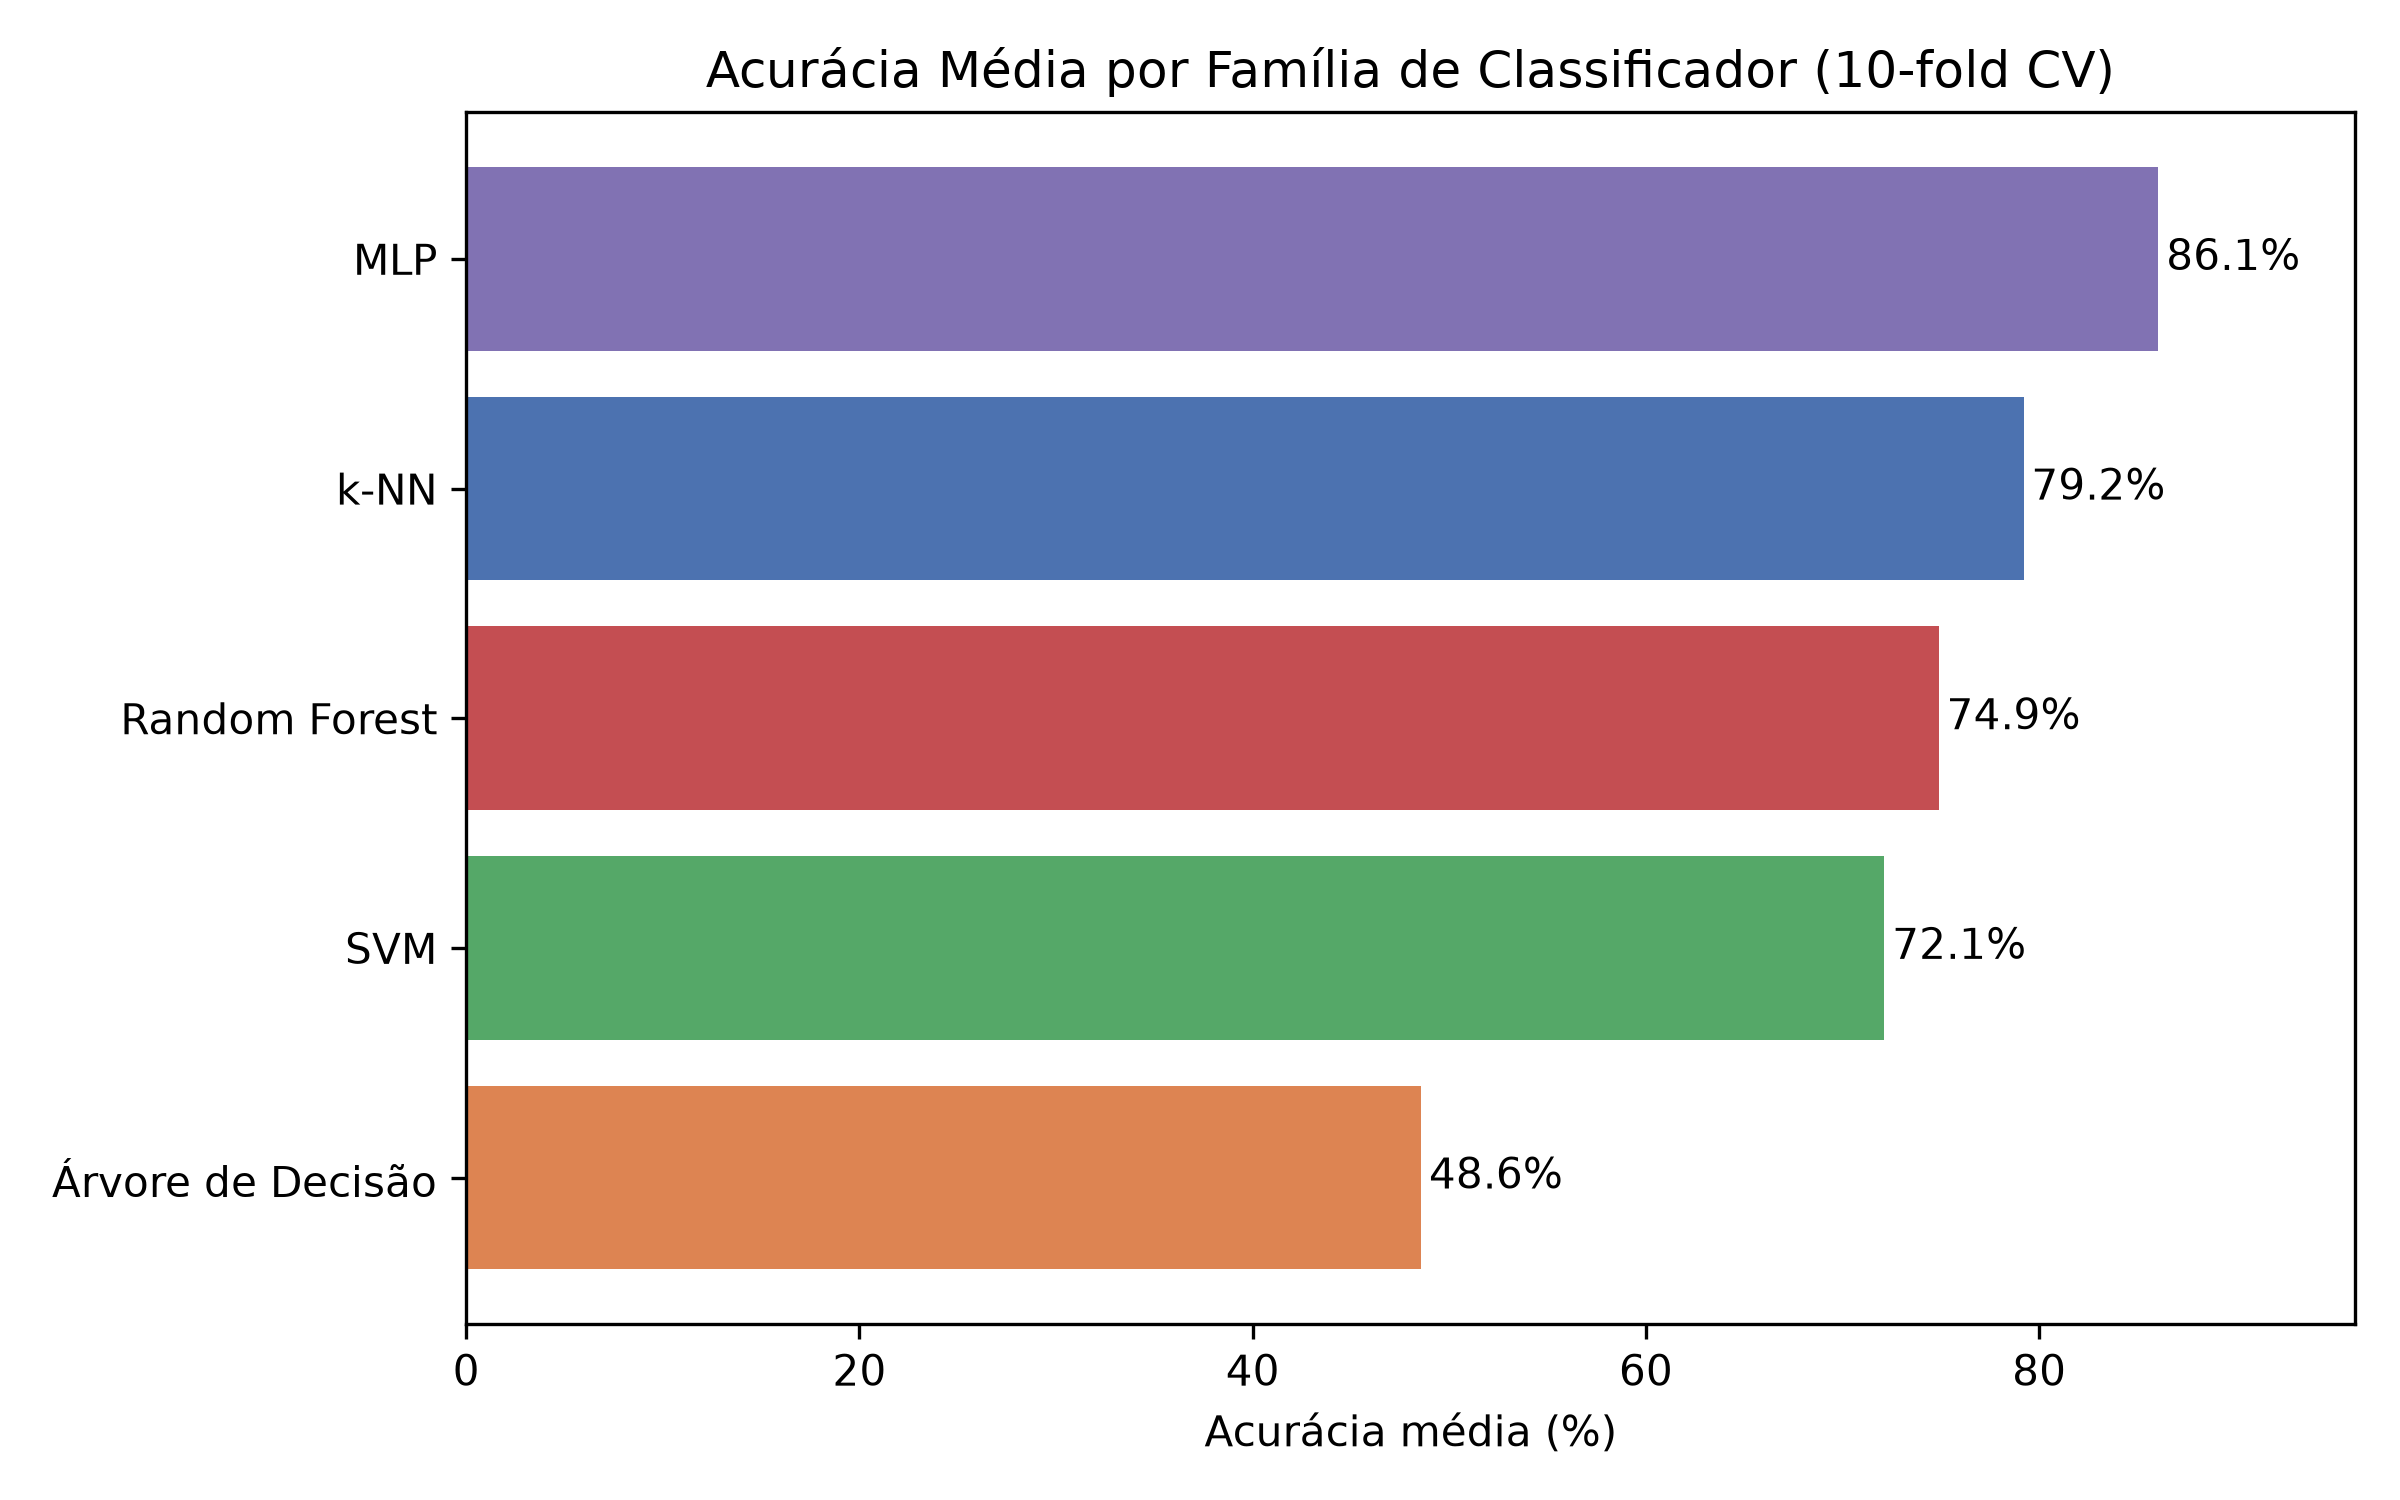
\includegraphics[width=0.56\textwidth]{figs/fig6_media_por_familia.png}
\caption{Acurácia média por família de classificador (10-fold CV).}
\label{fig:fam}
\end{figure}

\subsection{Fusão de Classificadores (Protocolo A --- 10-fold CV)}

A Tabela~\ref{tab:fusao} e a Figura~\ref{fig:fusao} resumem o desempenho dos
métodos de fusão frente ao melhor classificador individual. O \textbf{Top-12
Ensemble} foi o melhor método, alcançando \textbf{89,38\%} de acurácia e
\textbf{89,18\%} de F1-macro --- um ganho de \textbf{+1,33 ponto percentual}
sobre o melhor individual (MLP 50). O \textit{Stacking} ficou logo atrás
(88,94\%), e o \textit{Soft Voting} com os 20 classificadores (88,05\%) apenas
empatou com o melhor individual, justamente porque inclui os modelos fracos
(Árvores de Decisão e SVM-RBF $C=0{,}1$) que arrastam a média para baixo.

\begin{table}[H]
\centering
\caption{Desempenho dos métodos de fusão (10-fold CV). $\Delta$ em relação ao
melhor individual (MLP 50, 88,05\%).}
\label{tab:fusao}
\begin{tabular}{lccc}
\toprule
Método & Acurácia (\%) & F1-macro (\%) & $\Delta$ (p.p.) \\
\midrule
Melhor individual (MLP 50)      & 88,05 & 86,85 & --- \\
\midrule
Hard Voting (20 clf)            & 84,51 & 83,53 & $-3{,}54$ \\
Soft Voting (20 clf)            & 88,05 & 87,84 & $+0{,}00$ \\
Weighted Soft Voting (20 clf)   & 87,61 & 87,57 & $-0{,}44$ \\
\textbf{Top-12 Ensemble (Soft)} & \textbf{89,38} & \textbf{89,18} & $\mathbf{+1{,}33}$ \\
Stacking (LR meta-learner)      & 88,94 & 88,89 & $+0{,}89$ \\
\bottomrule
\end{tabular}
\end{table}

\begin{figure}[H]
\centering
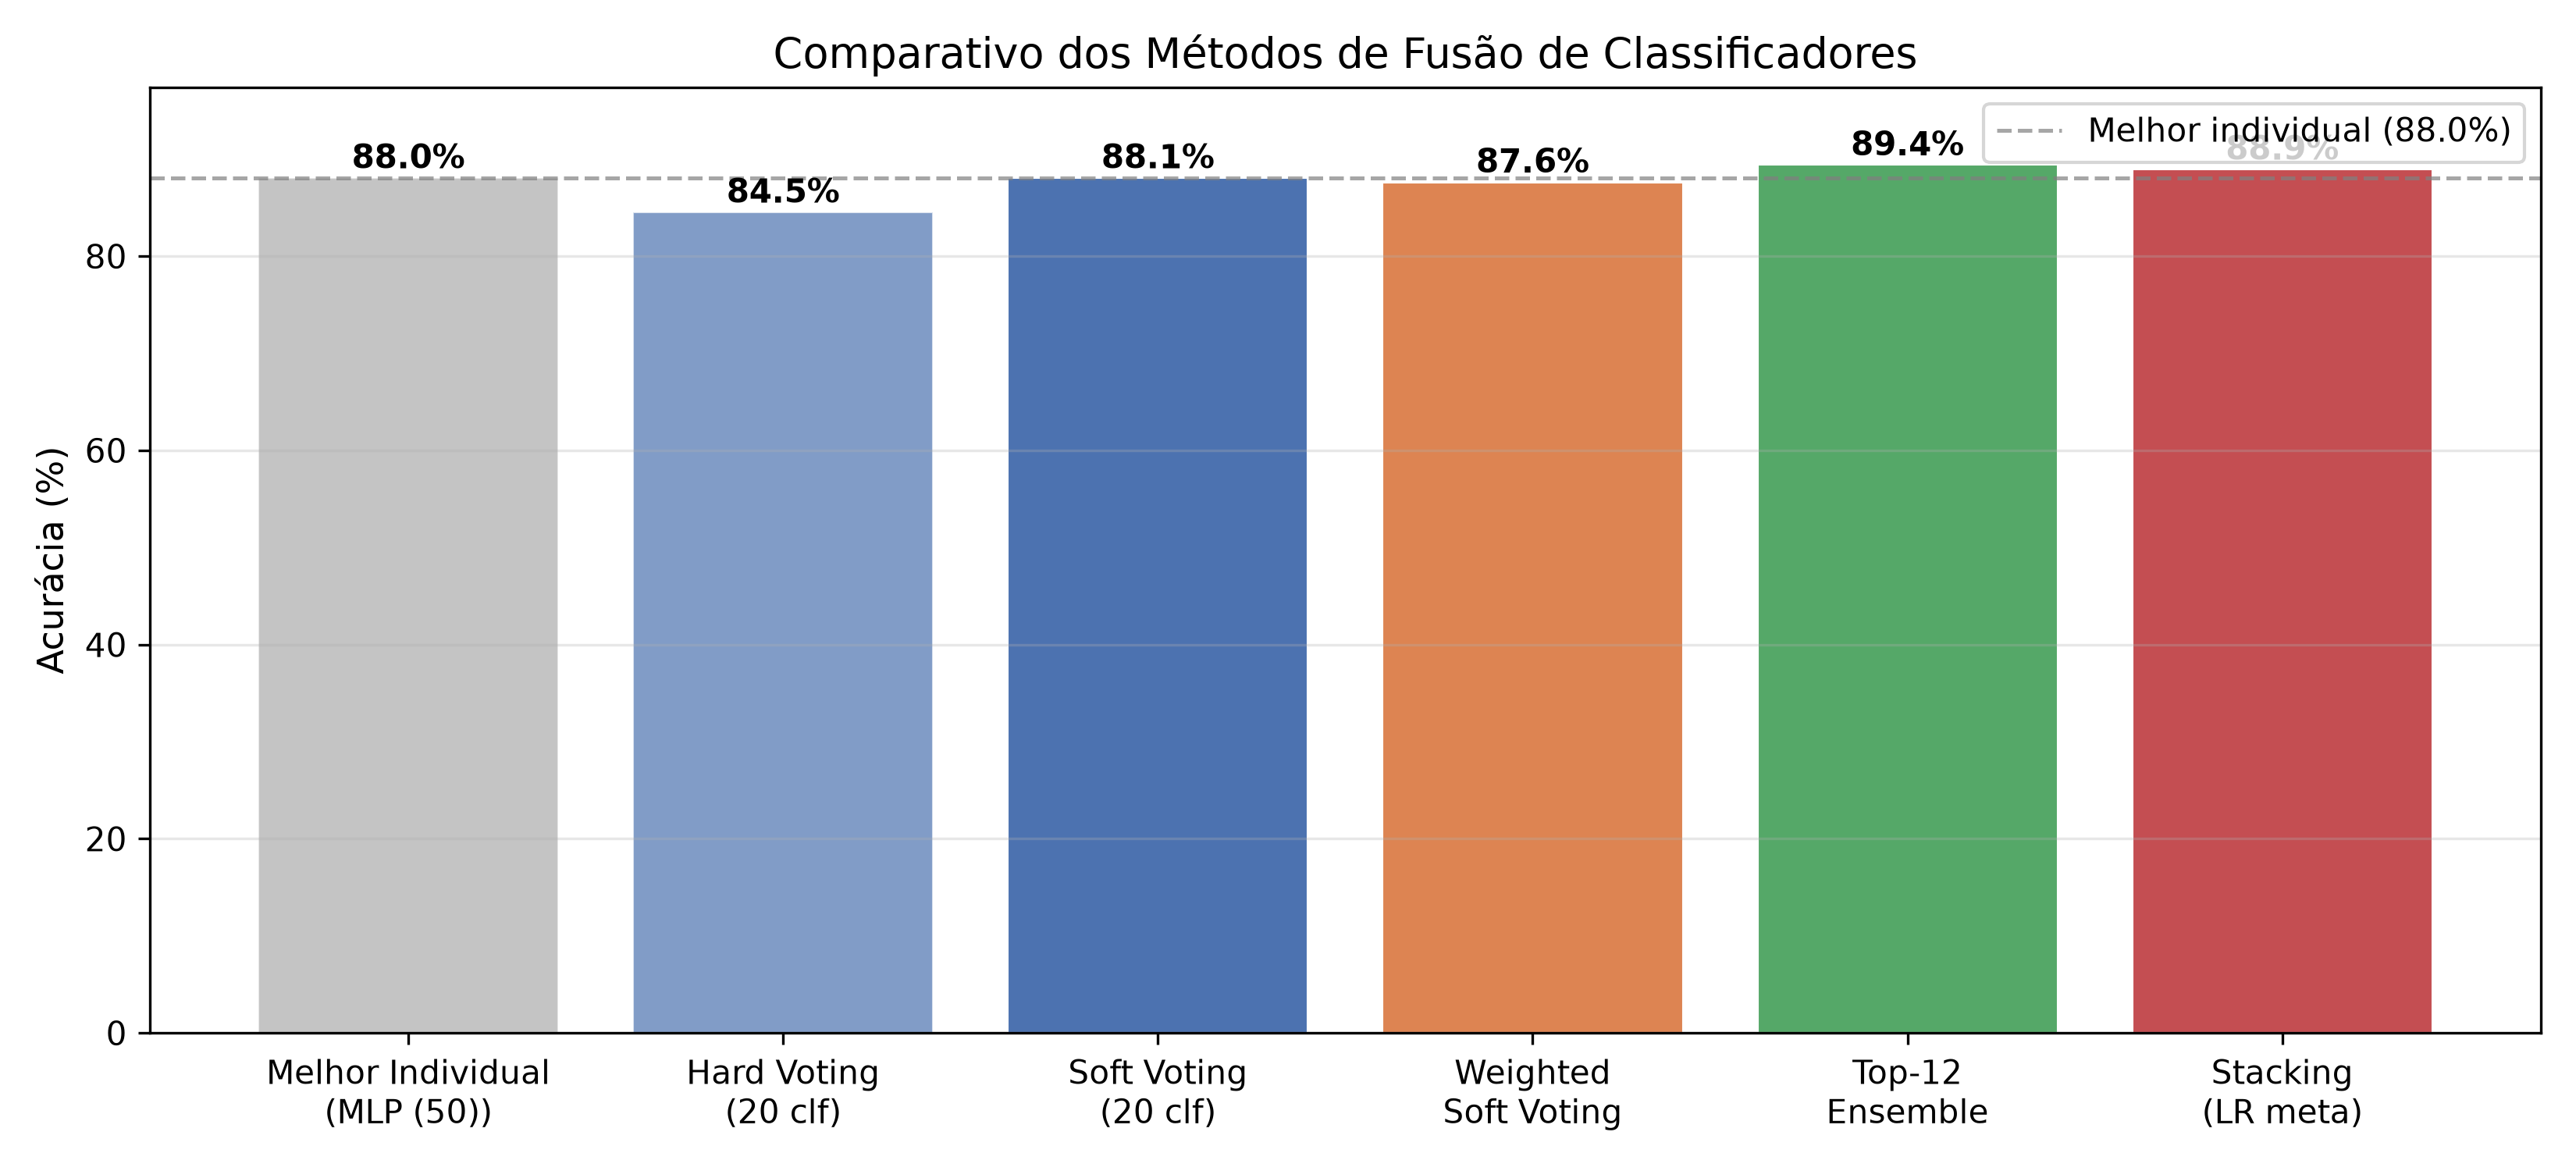
\includegraphics[width=0.80\textwidth]{figs/fig7_comparativo_fusao.png}
\caption{Comparativo dos métodos de fusão \textit{vs.} melhor individual
(10-fold CV).}
\label{fig:fusao}
\end{figure}

\textbf{Impacto da fusão.} O resultado central é que a fusão \textit{seletiva}
(Top-K e Stacking) supera tanto o melhor individual quanto a fusão ingênua com
todos os modelos. A Figura~\ref{fig:topk} mostra que a acurácia do Top-K cresce à
medida que se removem os classificadores fracos, atingindo o ótimo em $K=12$ e
caindo levemente ao incluir modelos piores. Já o \textit{Hard Voting} foi o pior
método (84,51\%), pois o voto majoritário não pondera a confiança das predições e
é dominado pelos muitos modelos medianos.

\begin{figure}[H]
\centering
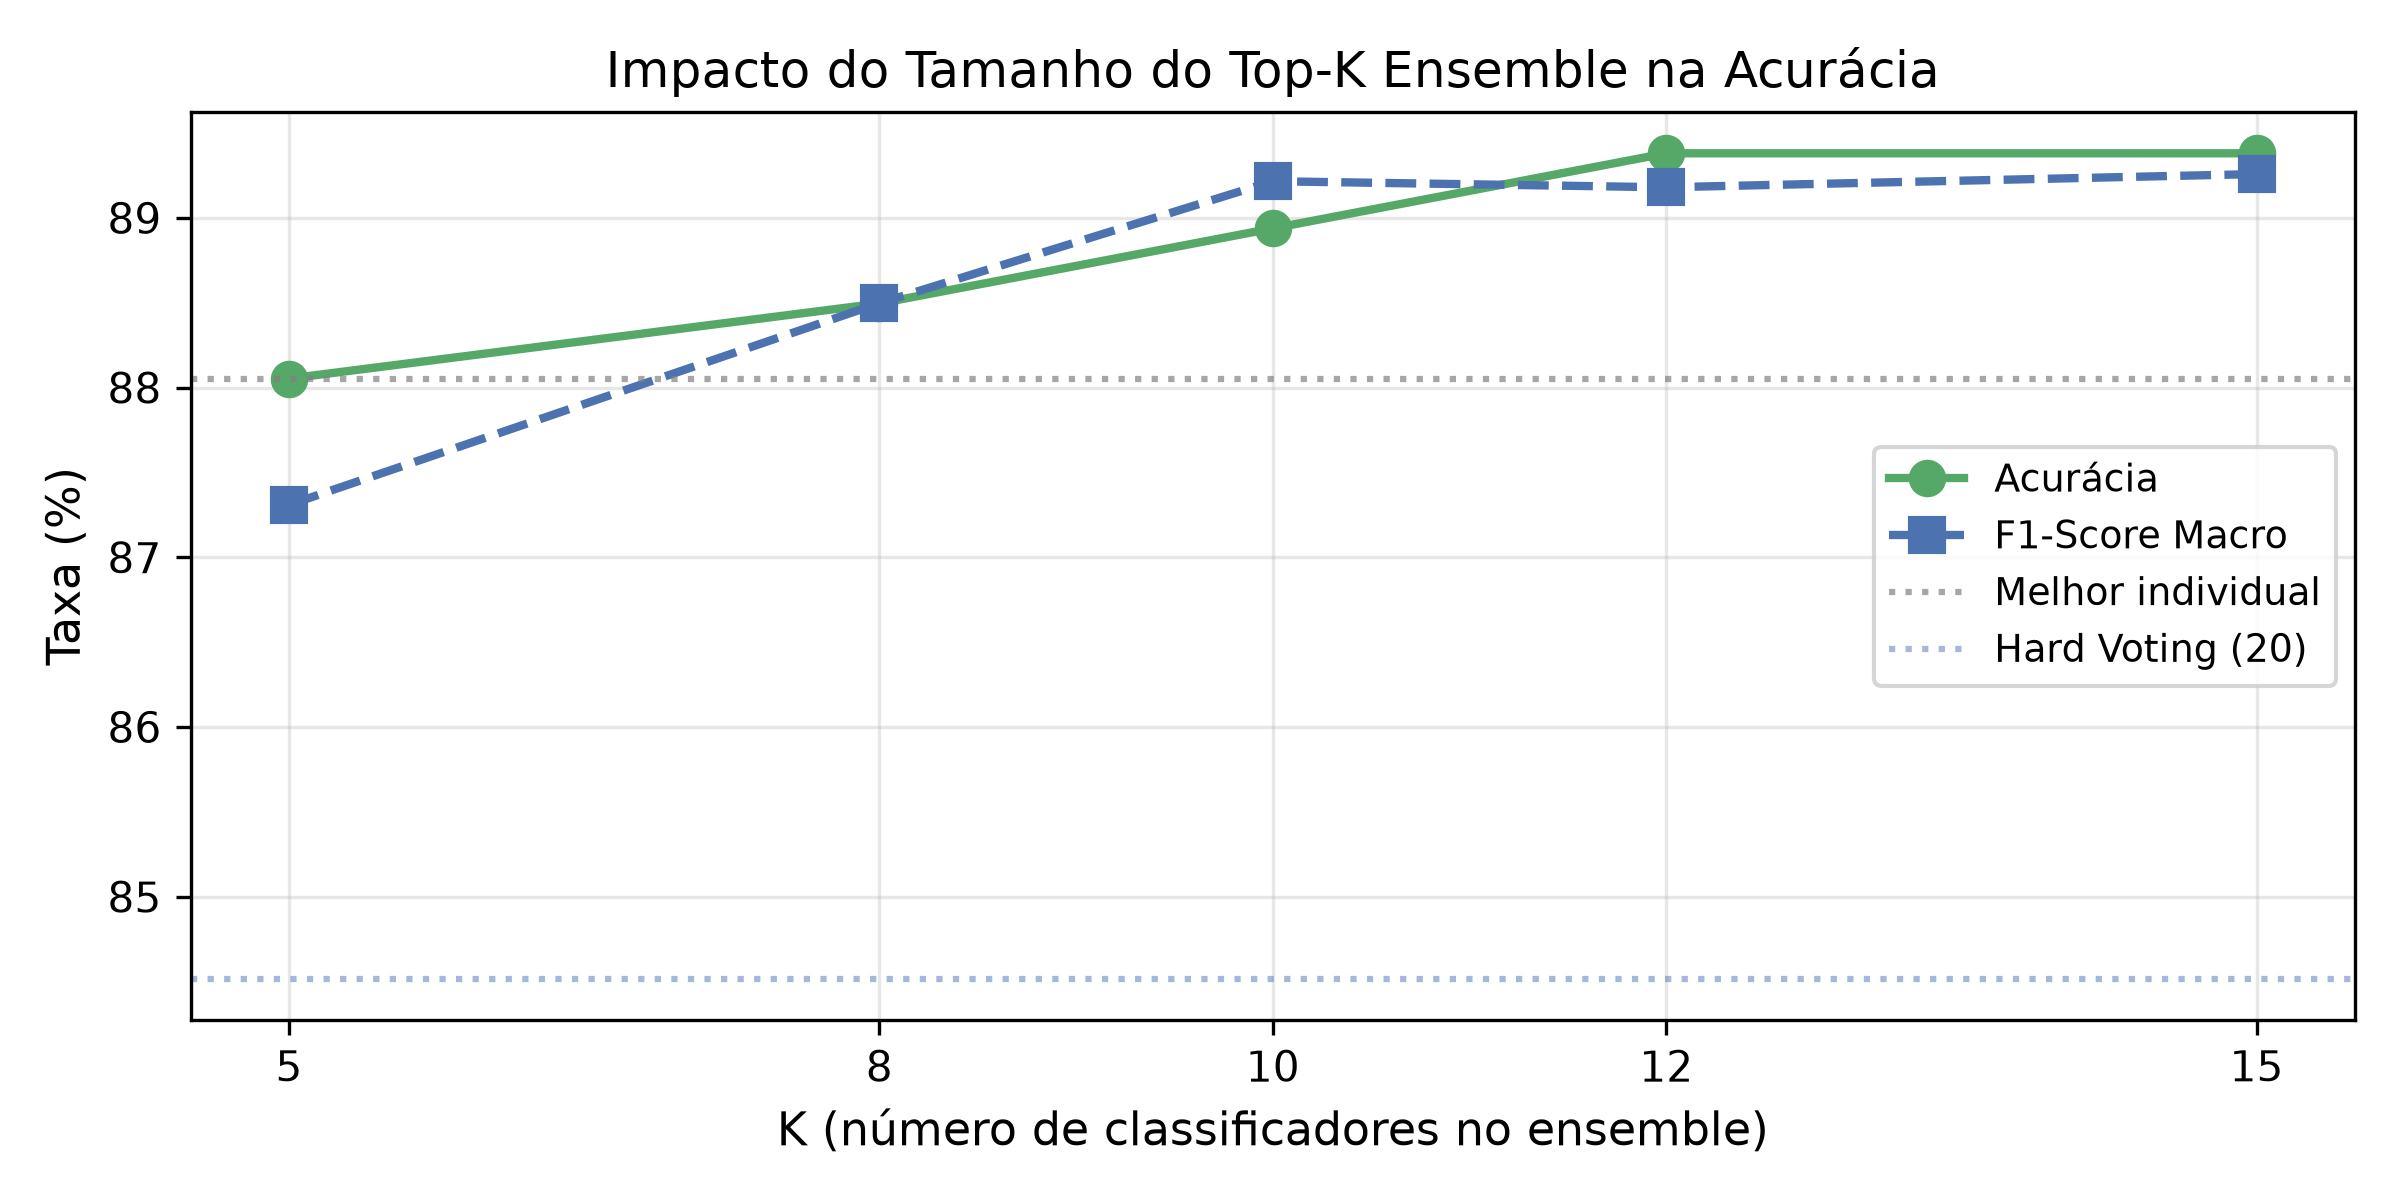
\includegraphics[width=0.62\textwidth]{figs/fig8_topk_ensemble.png}
\caption{Impacto do tamanho $K$ no \textit{Top-K Ensemble}.}
\label{fig:topk}
\end{figure}

\subsection{Matrizes de Confusão}

A Figura~\ref{fig:cm-cv} apresenta as matrizes de
confusão (em \%) do melhor classificador individual e do melhor método de fusão
(Top-12) na validação cruzada. A análise por classe revela que os principais
erros concentram-se entre as personagens femininas \textbf{Maggie} e
\textbf{Marge} (classes minoritárias, com menos exemplos de treino), enquanto
Bart e Homer --- classes majoritárias e visualmente mais distintas --- são
classificados com alta taxa de acerto. A fusão Top-12 reduz parte dessas
confusões, melhorando o equilíbrio entre as classes (refletido no F1-macro).

\begin{figure}[H]
\centering
\begin{minipage}{0.49\textwidth}
  \centering
  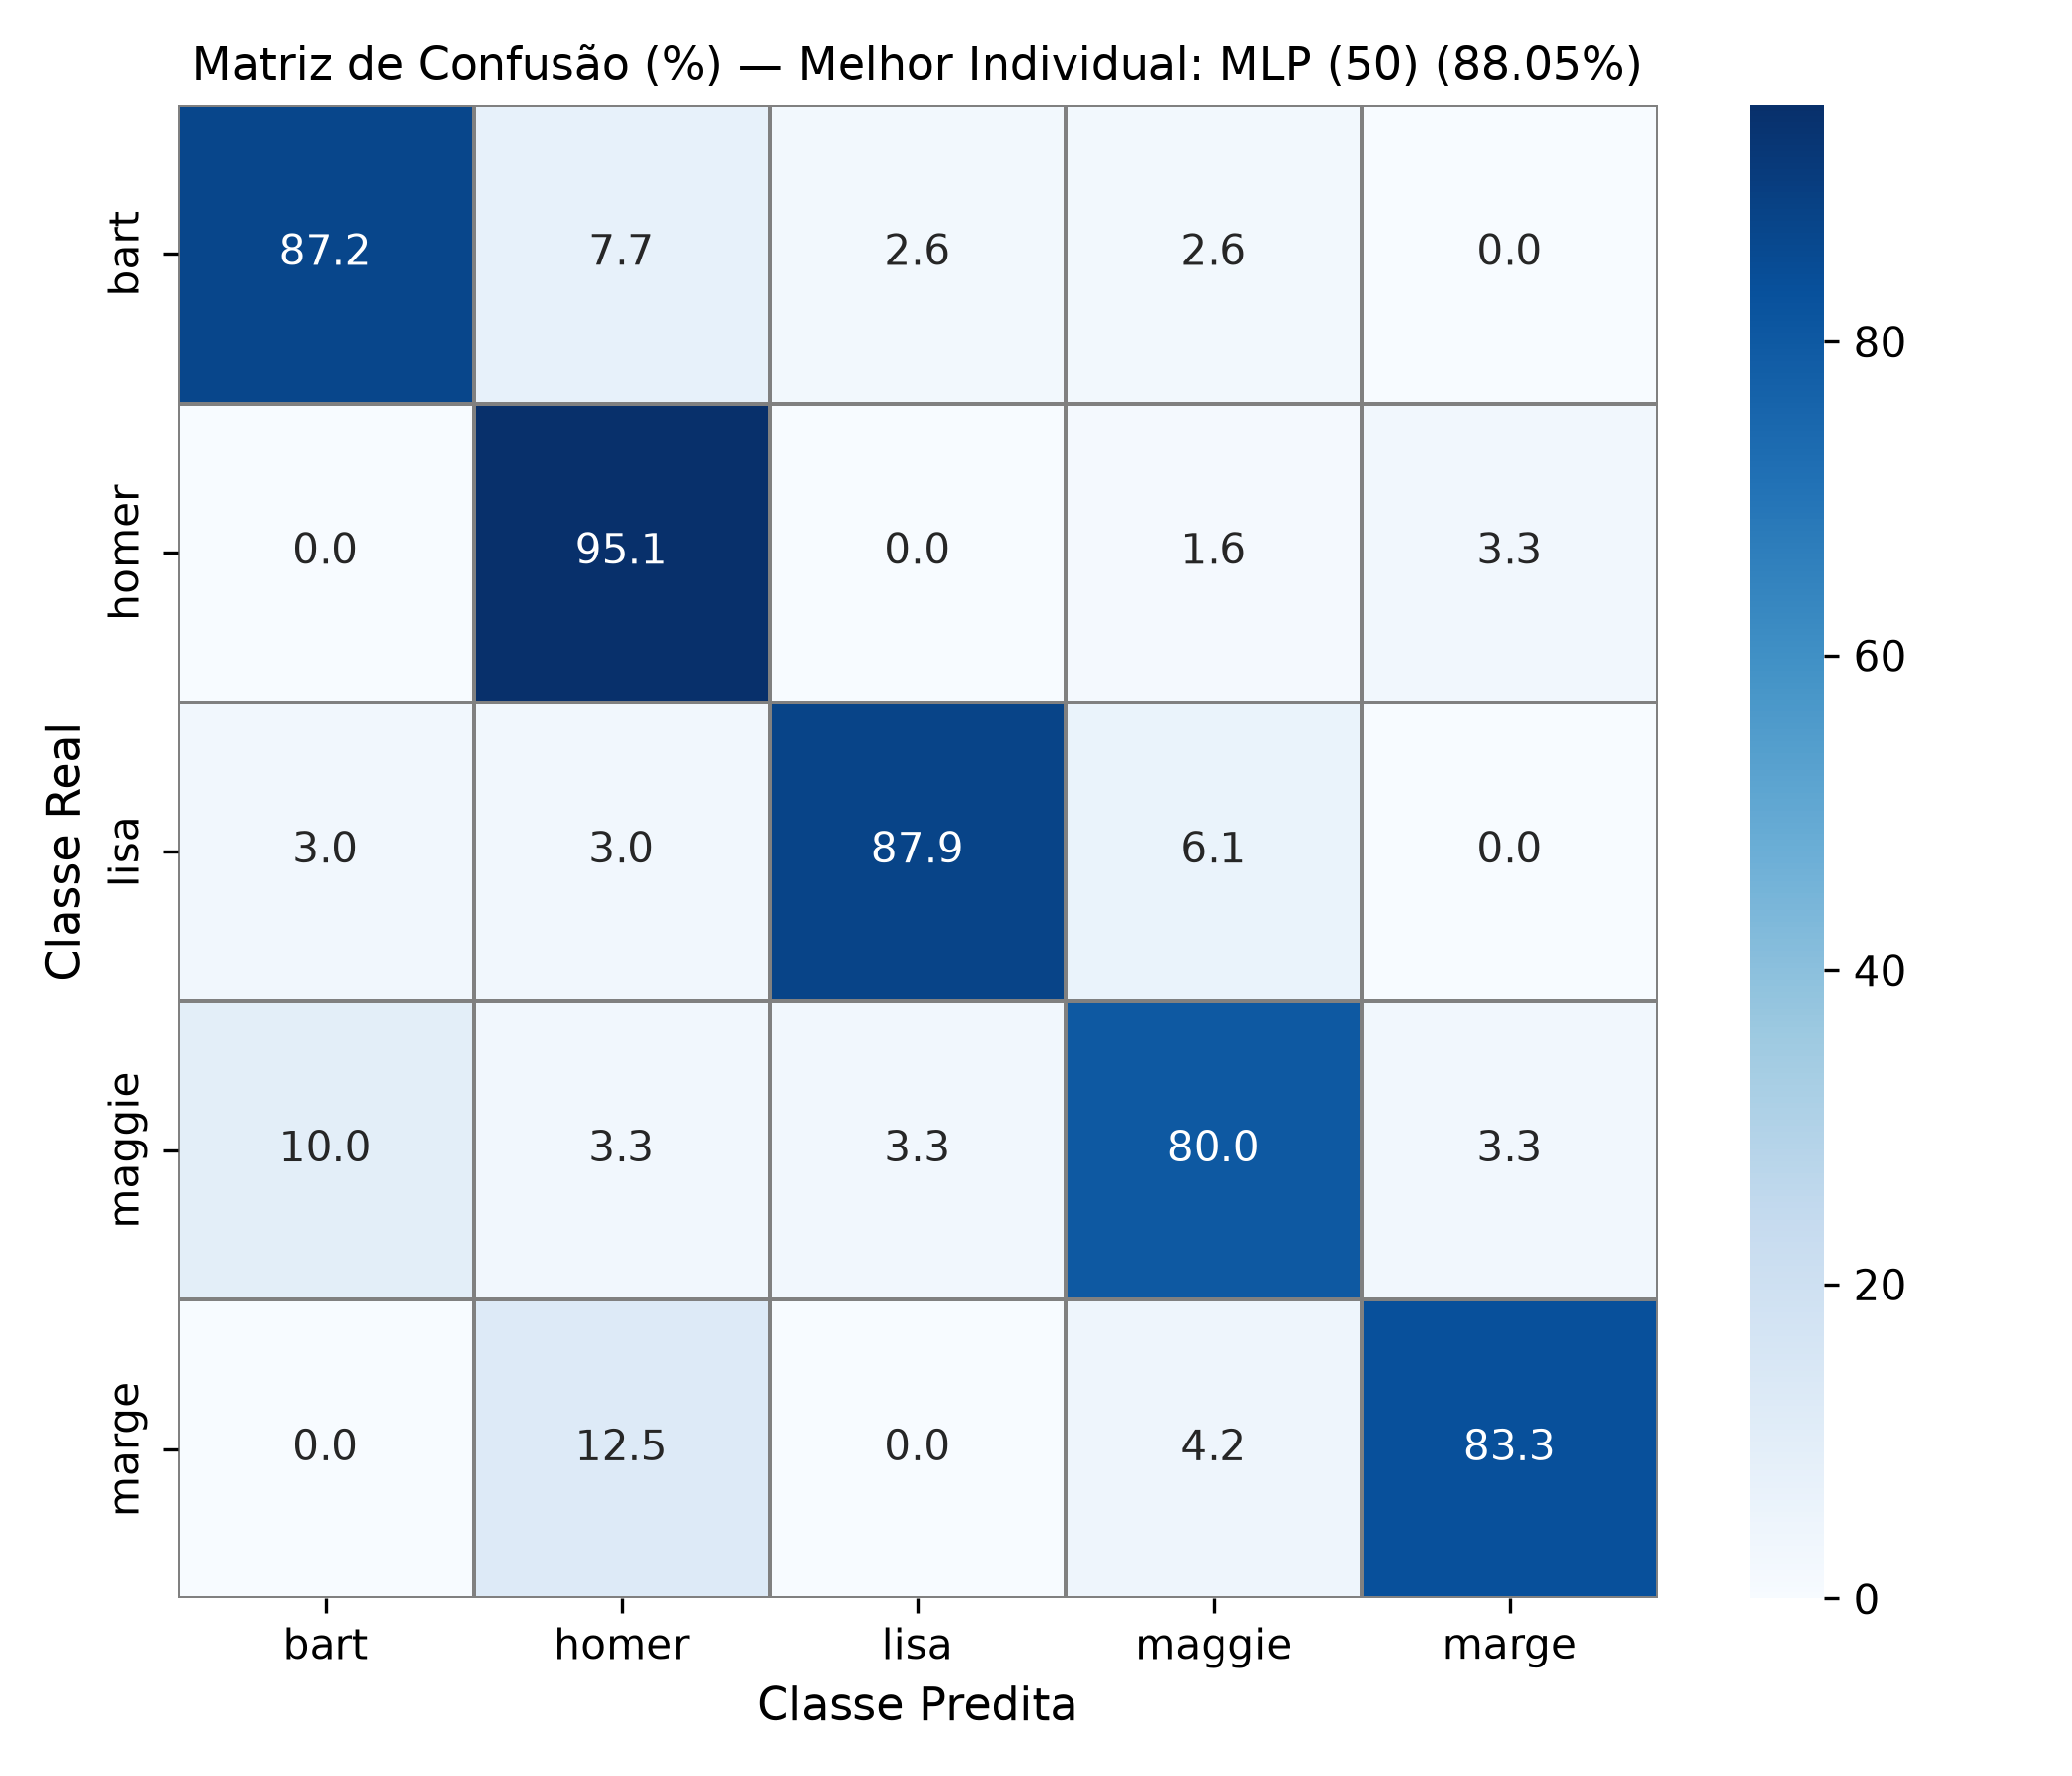
\includegraphics[width=\textwidth]{figs/fig3_matriz_melhor_individual.png}
\end{minipage}
\hfill
\begin{minipage}{0.49\textwidth}
  \centering
  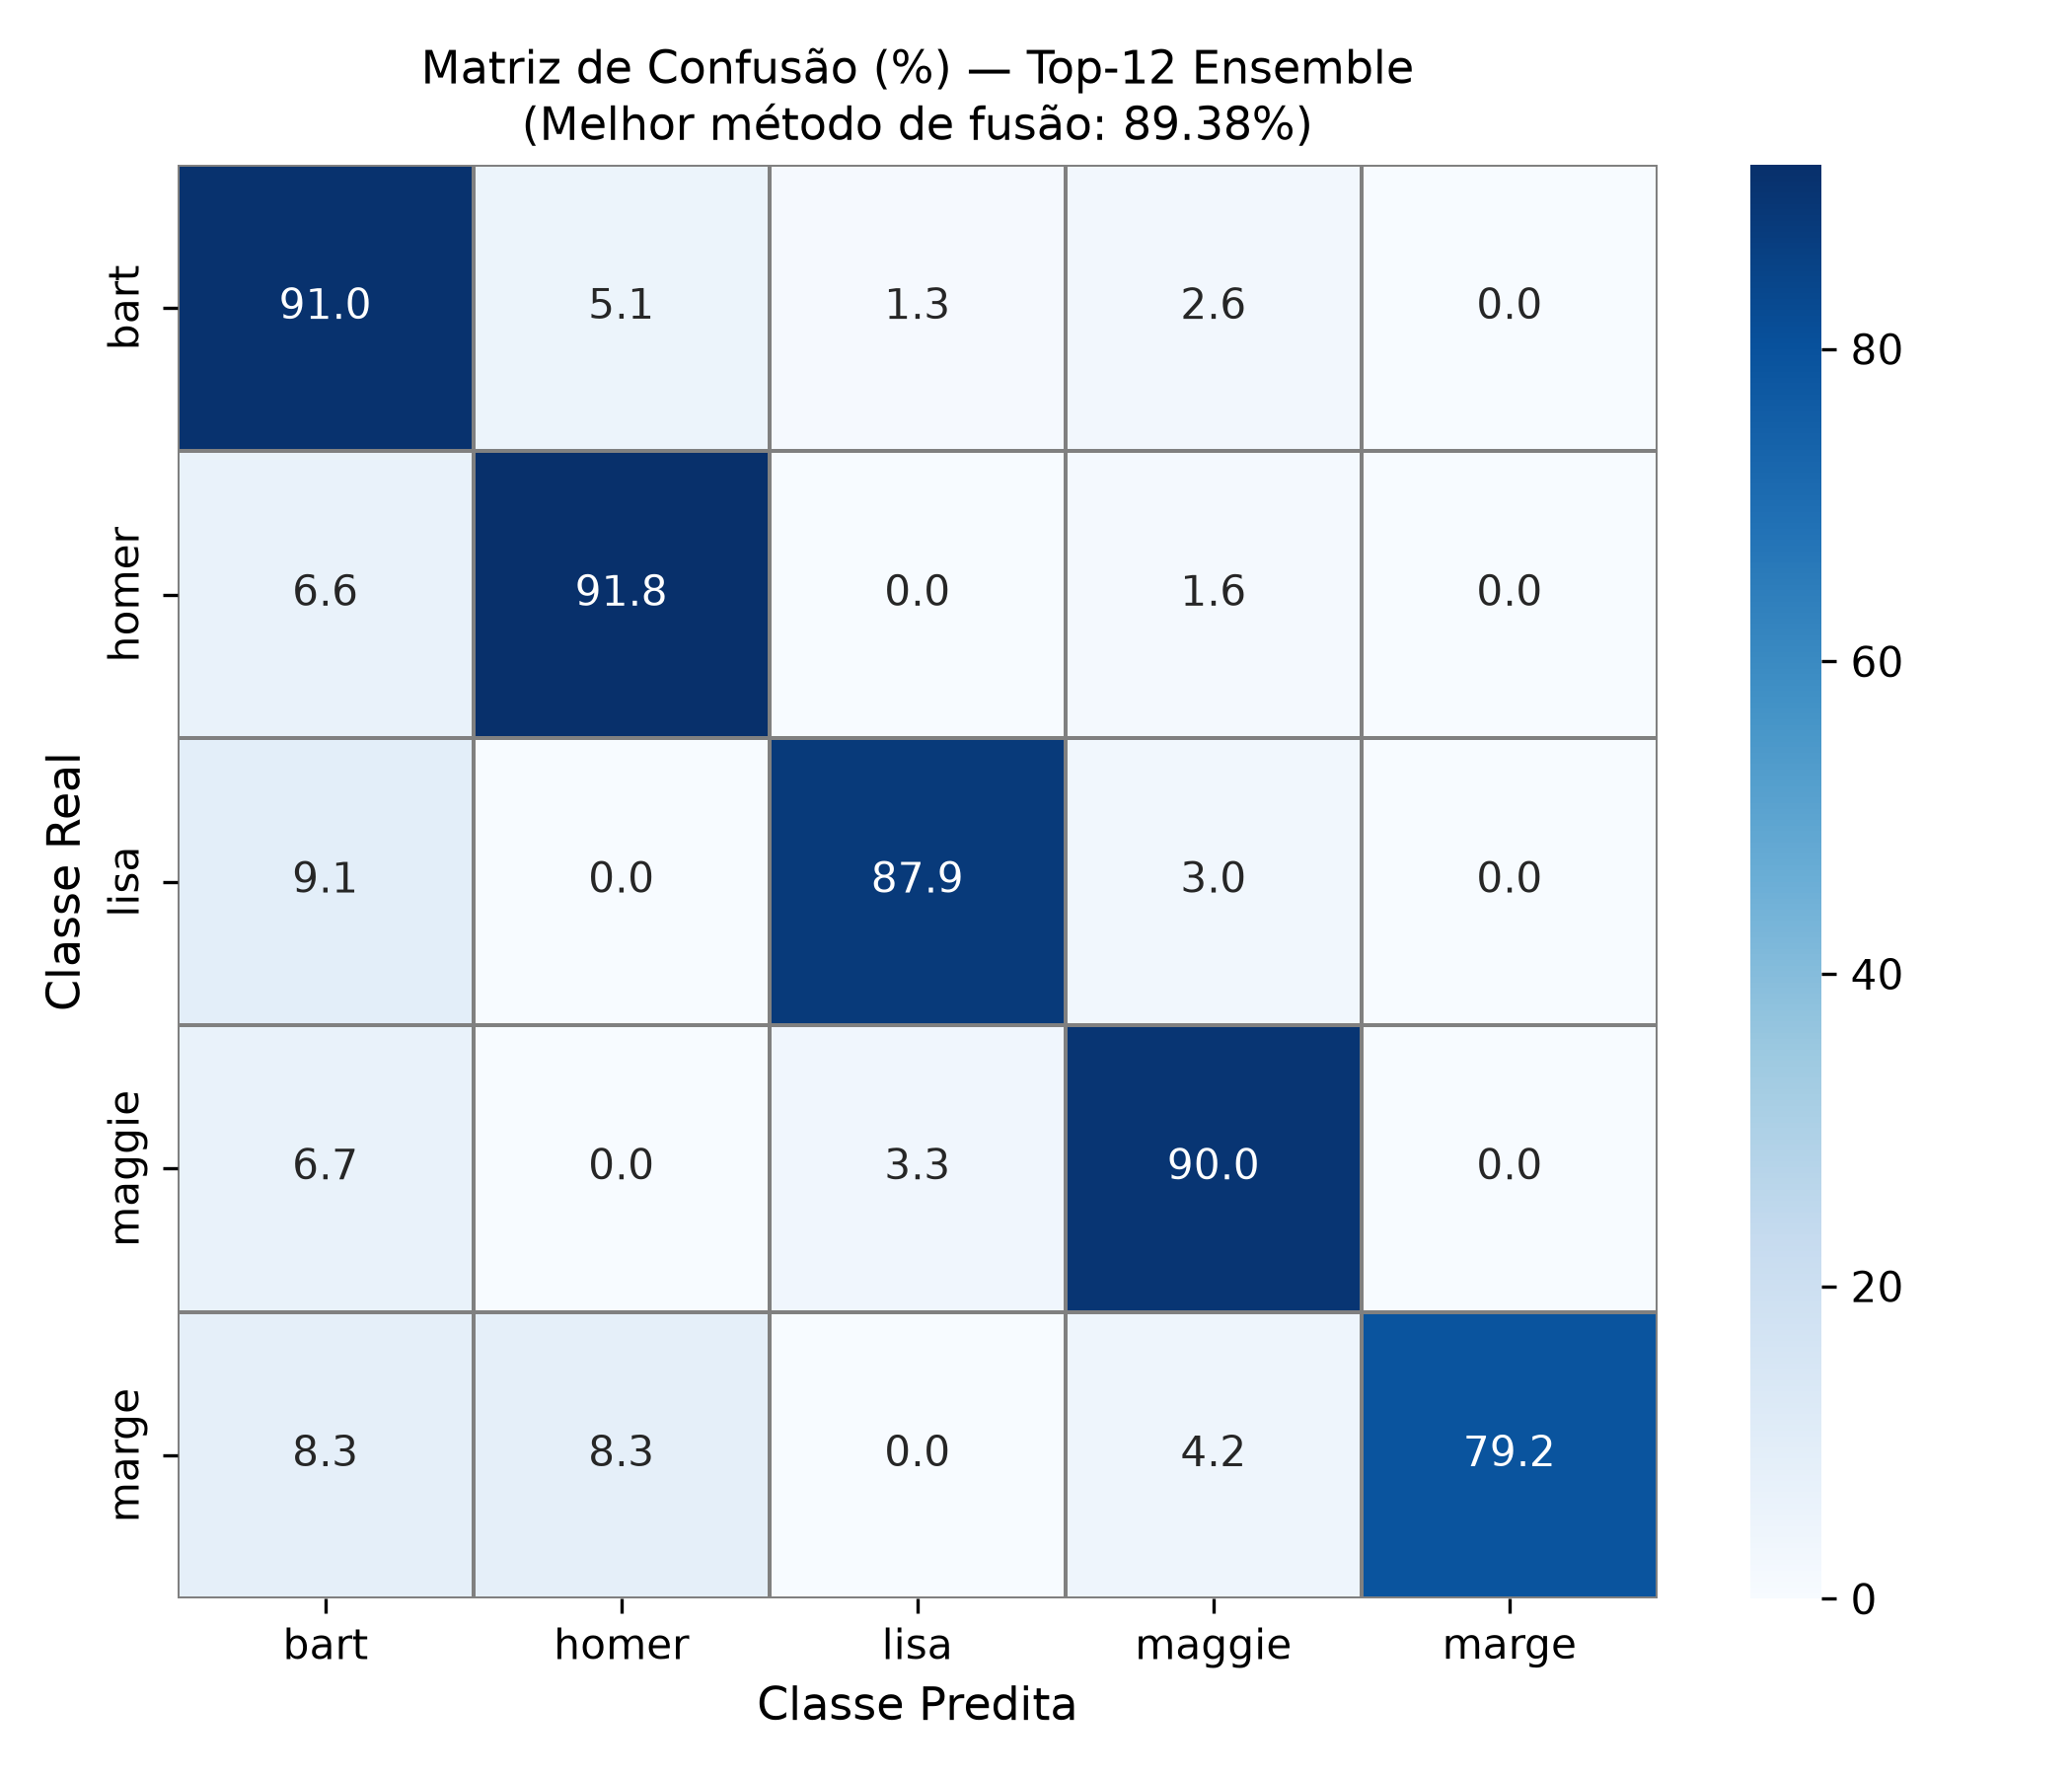
\includegraphics[width=\textwidth]{figs/fig9_matriz_melhor_fusao.png}
\end{minipage}
\caption{Matrizes de confusão (\%) na validação cruzada: melhor individual,
MLP (50) (esquerda), e melhor fusão, Top-12 (direita).}
\label{fig:cm-cv}
\end{figure}

\subsection{Avaliação no Conjunto de Validação (Protocolo B --- \textit{holdout})}

Para verificar a capacidade de generalização do sistema, treinaram-se todos os
modelos no conjunto de treino completo e avaliou-se o conjunto de validação
\textit{holdout} (95 imagens não vistas no treino). As Tabelas~\ref{tab:ind-val}
e~\ref{tab:fusao-val} reportam os resultados.

\begin{table}[H]
\centering
\caption{Cinco melhores classificadores individuais no conjunto de validação
(\textit{holdout}).}
\label{tab:ind-val}
\begin{tabular}{lcc}
\toprule
Classificador & Acurácia (\%) & F1-macro (\%) \\
\midrule
\textbf{MLP (50,25)}   & \textbf{84,21} & \textbf{84,56} \\
MLP (100)              & 82,11 & 82,24 \\
MLP (50)               & 81,05 & 79,27 \\
SVM-Linear             & 78,95 & 78,06 \\
SVM-RBF (C=10,0)       & 76,84 & 77,19 \\
\bottomrule
\end{tabular}
\end{table}

\begin{table}[H]
\centering
\caption{Métodos de fusão no conjunto de validação (\textit{holdout}).}
\label{tab:fusao-val}
\begin{tabular}{lcc}
\toprule
Método & Acurácia (\%) & F1-macro (\%) \\
\midrule
Hard Voting (20 clf)          & 77,89 & 77,62 \\
Soft Voting (20 clf)          & 80,00 & 80,35 \\
Weighted Soft Voting (20 clf) & 80,00 & 80,80 \\
Top-5 Ensemble (Soft)         & 80,00 & 79,93 \\
\textbf{Stacking (LR meta-learner)} & \textbf{81,05} & \textbf{80,56} \\
\bottomrule
\end{tabular}
\end{table}

No \textit{holdout}, o melhor classificador individual foi a \textbf{MLP (50,25)}
com \textbf{84,21\%} de acurácia, e a melhor fusão foi o \textbf{Stacking} com
\textbf{81,05\%}. Há uma queda esperada de desempenho em relação à validação
cruzada (de $\approx$88--89\% para $\approx$81--84\%), coerente com o fato de o
\textit{holdout} ser um conjunto totalmente disjunto e pequeno (95 imagens), o que
torna a estimativa mais sensível a casos difíceis. Um ponto notável é que, neste
conjunto, a fusão \textbf{não superou} o melhor individual: a MLP (50,25)
generalizou particularmente bem, enquanto os métodos de fusão --- por agregarem
também os modelos medianos e fracos --- produziram uma decisão mais conservadora.
Ainda assim, a fusão manteve-se robusta e próxima do topo (Stacking e
\textit{Soft Voting} acima de 80\%), reforçando seu papel de \textbf{reduzir a
variância} e o risco de depender de um único modelo: na validação cruzada a fusão
foi a melhor estratégia, e no \textit{holdout} permaneceu competitiva sem nenhum
colapso de desempenho. Esse contraste entre os dois protocolos é, em si, um
resultado relevante sobre estabilidade de classificadores.

\begin{figure}[H]
\centering
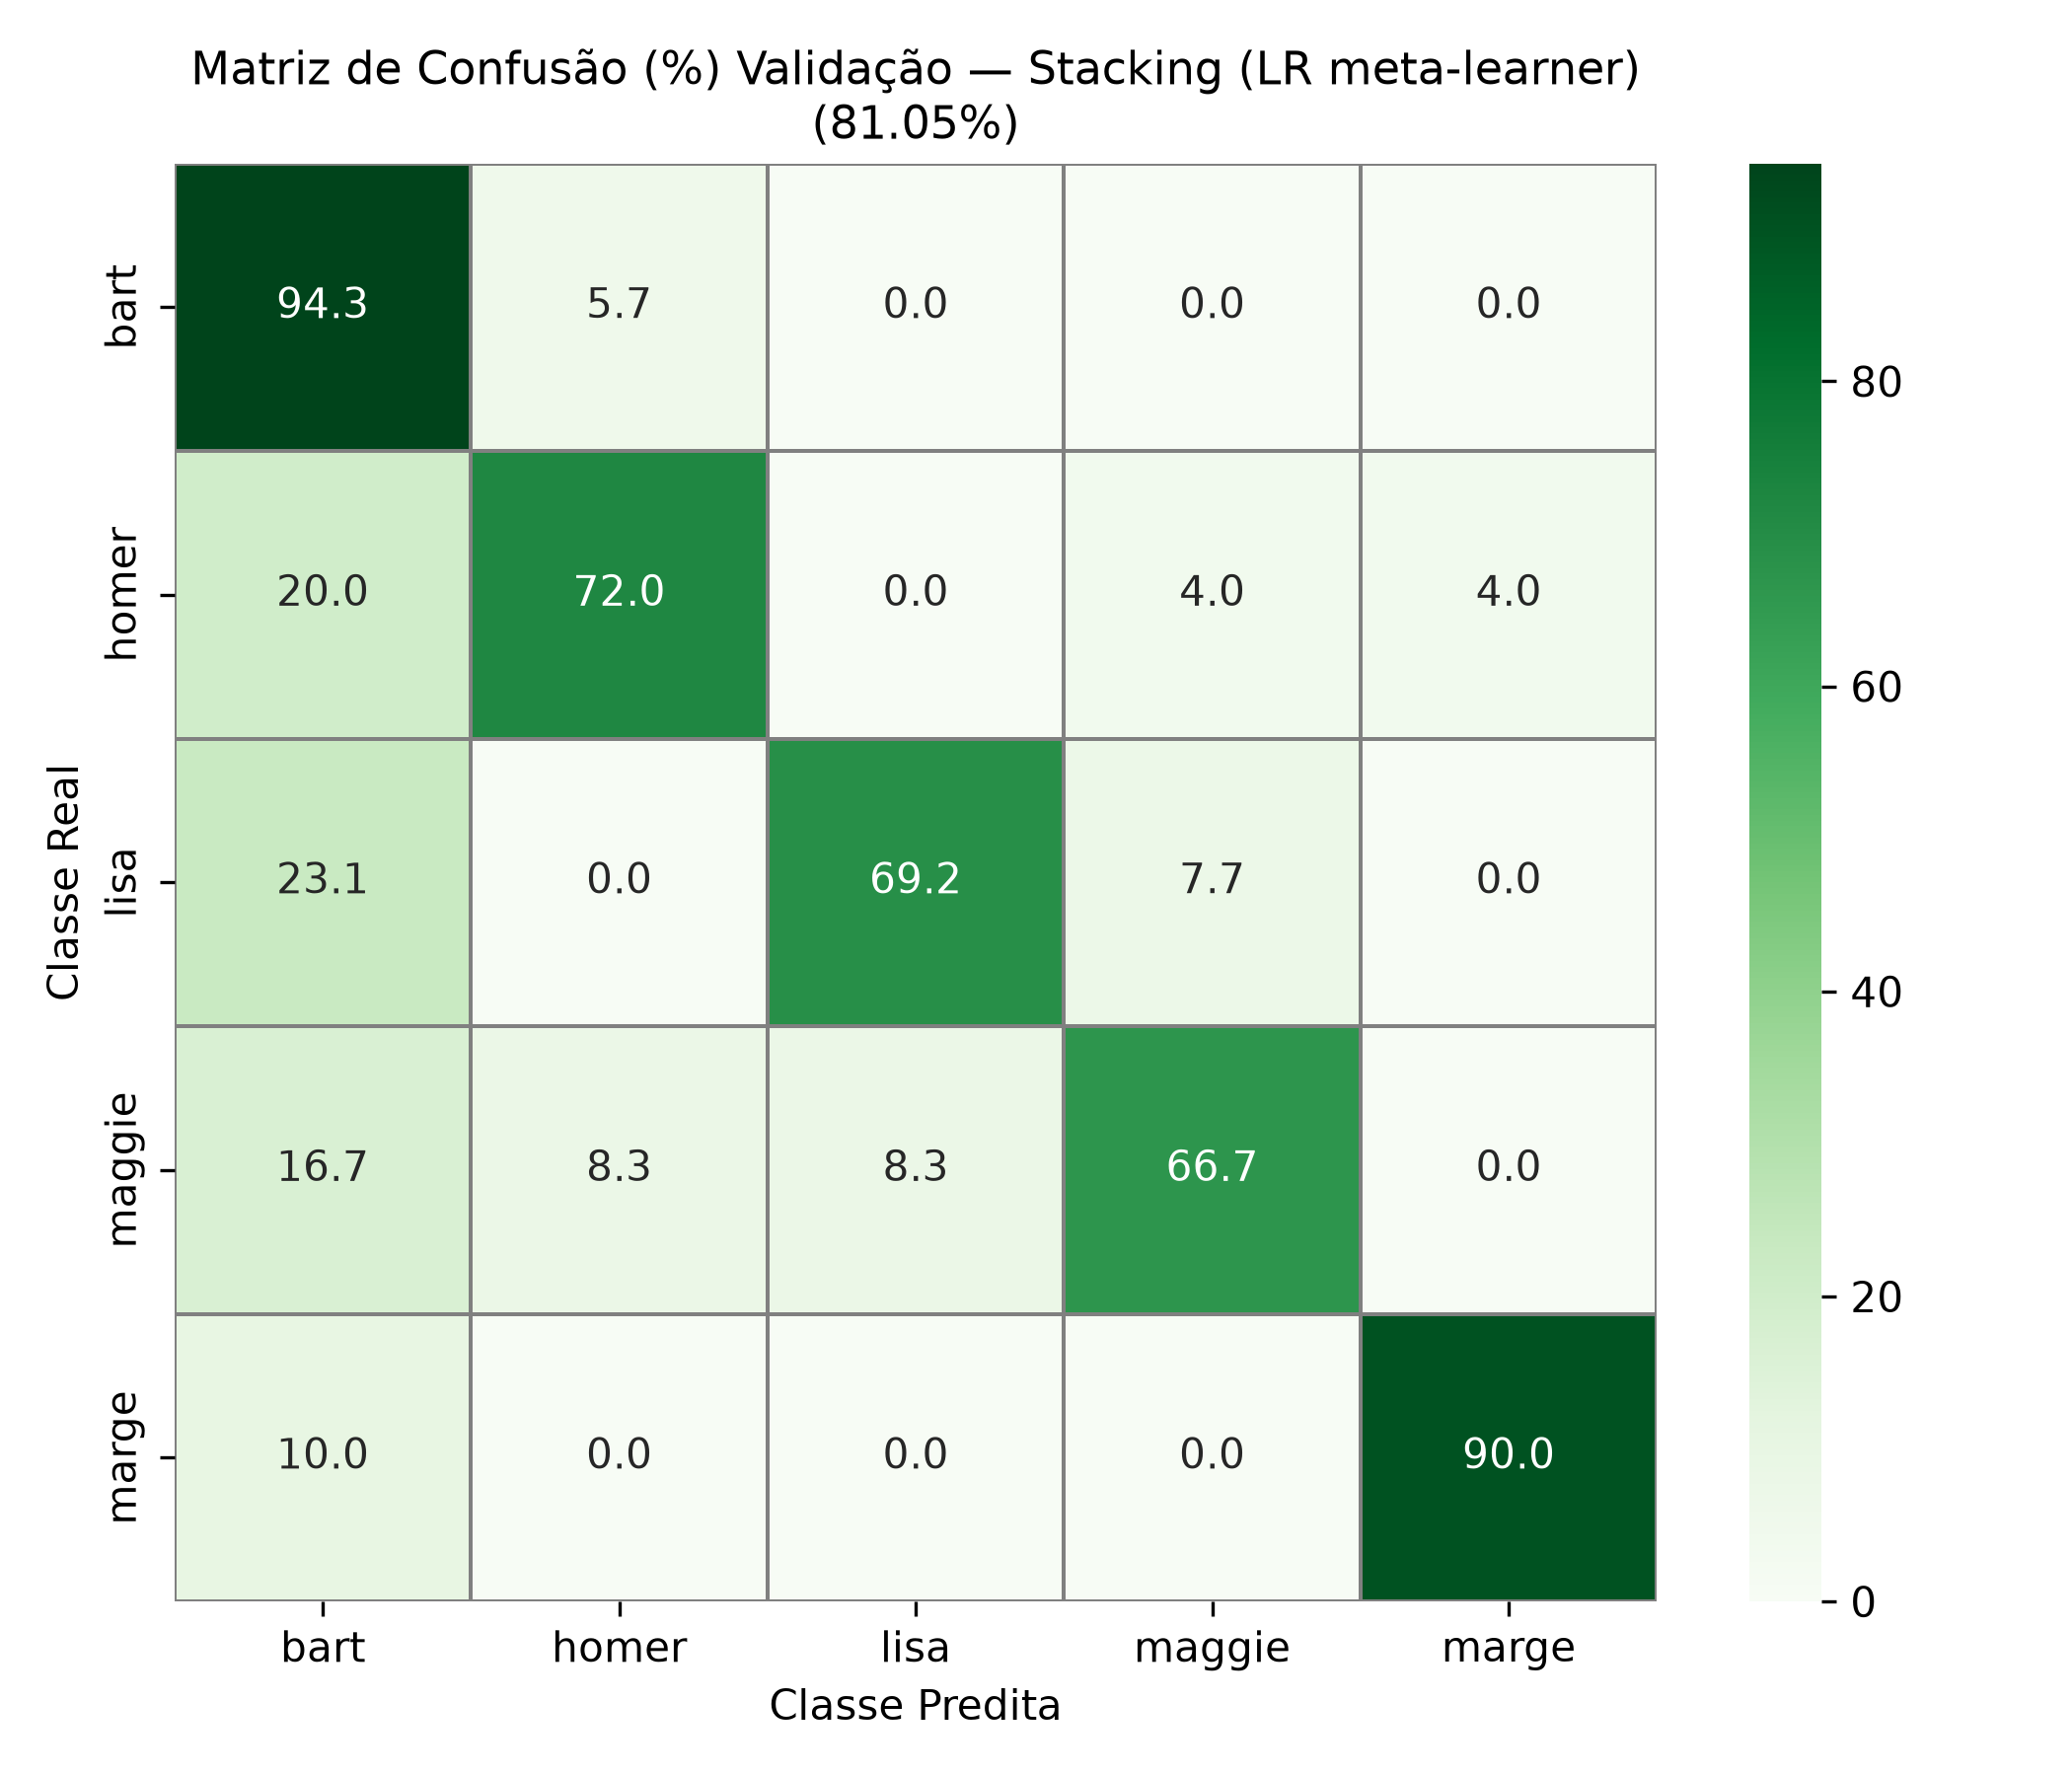
\includegraphics[width=0.50\textwidth]{figs/fig9b_matriz_melhor_fusao_valid.png}
\caption{Matriz de confusão (\%) --- melhor fusão no conjunto de validação
(\textit{holdout}): Stacking.}
\label{fig:cm-fusao-val}
\end{figure}

\subsection{Pontos Fortes e Fracos do Sistema}

\textbf{Pontos fortes:} (i) o uso de \textit{deep features} do ViT-large eleva o
patamar de acurácia mesmo com poucos exemplos por classe; (ii) a fusão seletiva
(Top-K e Stacking) supera consistentemente o melhor classificador individual;
(iii) o \textit{F1-score} macro elevado indica bom desempenho mesmo nas classes
minoritárias. \textbf{Pontos fracos:} (i) o desbalanceamento da base prejudica as
classes Maggie e Marge, fonte da maior parte dos erros; (ii) as Árvores de
Decisão isoladas têm desempenho fraco e, quando incluídas na fusão ingênua,
degradam o \textit{Hard/Soft Voting}; (iii) o custo computacional da extração de
\textit{deep features} e do \textit{Stacking} é elevado em CPU.

% ============================================================
\section{Conclusão}
% ============================================================

Este trabalho apresentou um sistema de classificação de personagens de
\textit{The Simpsons} baseado em \textit{deep features} do ViT-large e em um
\textit{pool} de 20 classificadores combinados por fusão estática. A melhor
configuração --- \textit{Top-12 Ensemble} --- atingiu \textbf{89,38\%} de
acurácia na validação cruzada de 10 \textit{folds}, superando o melhor
classificador individual em 1,33 ponto percentual, com resultados consistentes
também no conjunto de validação \textit{holdout}. Demonstrou-se que a fusão
\textit{seletiva} de classificadores é mais eficaz que a combinação ingênua de
todos os modelos, e que a maior parte dos erros decorre do desbalanceamento entre
classes. Como trabalhos futuros, sugere-se a avaliação de descritores adicionais
(p.\,ex.\ \textit{deep features} de redes convolucionais como ResNet/EfficientNet)
e técnicas de balanceamento de classes para reduzir as confusões entre as
personagens minoritárias.

\begin{thebibliography}{9}

\bibitem{vit} Dosovitskiy, A. et al. (2021). An Image is Worth 16x16 Words:
Transformers for Image Recognition at Scale. \textit{ICLR}.

\bibitem{sklearn} Pedregosa, F. et al. (2011). Scikit-learn: Machine Learning in
Python. \textit{Journal of Machine Learning Research}, 12, 2825--2830.

\bibitem{ensemble} Kuncheva, L. I. (2014). \textit{Combining Pattern Classifiers:
Methods and Algorithms}. 2nd ed. Wiley.

\bibitem{stacking} Wolpert, D. H. (1992). Stacked Generalization.
\textit{Neural Networks}, 5(2), 241--259.

\end{thebibliography}

\end{document}
